\subsubsection{XML Import}
\par
The general idea with this utility is to import XML files into the a configured database. This will take any xml file or input stream convert them into java objects and then store them into an SQL database. The interface to this utility is an intiutive user interface where you can open, preview and import files. 

\begin{figure}[h]
	\centering
		\includegraphics[width=3.00in]{ImportUse.jpg}
	\caption{The Use Case For The Import Utility}
	\label{fig:Import Use}
\end{figure}
\par
The import panel is a java swing JPanel. I included a text area for previewing files before importing. You can open the files that you want to import with the open button. This button brings up an open dialog that has a default filter for xml files. Once opened the file can be previewed by pressing the preview button or imported using the import button. The import utility assumes that you have already set up your database. Any error message you receive are likely because the database or hibernate properties have not been configured correctly. 


\par
The XML Import module is made up of two classes: the ImportPanel, and the ImportEngine. I chose this design to have interface seperated from functionality. I wanted the ImportEngine to be removable from the GUI so developers can take that class and use it with other user interfaces. 

\begin{figure}[h]
	\centering
		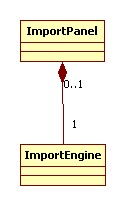
\includegraphics[width=1.00in]{ImportClasses.jpg}
	\caption{The ImportEngine is part of the ImportPanel but it can also run stand-alone}
	\label{fig:ImportClasses}
\end{figure}

When the import button is pressed a new ImportEngine is created. The ImportEngine takes a hibernate configuration and a JaxB context path. 

